%!TEX root = ../report.tex

%%%%%%%%%%%%%%%%%%%%%%%%%%%%%%%%%%%%%%%%%%%%%%%%%%%%%%%%%%%
\chapter{Analyse \label{analyse_analyse}}
%%%%%%%%%%%%%%%%%%%%%%%%%%%%%%%%%%%%%%%%%%%%%%%%%%%%%%%%%%%

her vil jeg.. Lorem ipsum dolor sit amet, consectetur adipisicing elit, sed do eiusmod
tempor incididunt ut labore et dolore magna aliqua. Ut enim ad minim veniam,
quis nostrud exercitation ullamco laboris nisi ut aliquip ex ea commodo
consequat. Duis aute irure dolor in reprehenderit in voluptate velit esse
cillum dolore eu fugiat nulla pariatur. Excepteur sint occaecat cupidatat non
proident, sunt in culpa qui officia deserunt mollit anim id est laborum. 

%%%%%%%%%%%%%%%%%%%%%%%%%%%%%%%%%%%%%%%%%%%%%%%%%%%%%%%%%%%
\chapter{Delanalyse 1: delmarkeder og segmenter, noget i den retning \label{analyse_deskriptivt}}
%%%%%%%%%%%%%%%%%%%%%%%%%%%%%%%%%%%%%%%%%%%%%%%%%%%%%%%%%%%

Lorem ipsum dolor sit amet, consectetur adipisicing elit, sed do eiusmod
tempor incididunt ut labore et dolore magna aliqua. Ut enim ad minim veniam,
quis nostrud exercitation ullamco laboris nisi ut aliquip ex ea commodo
consequat. Duis aute irure dolor in reprehenderit in voluptate velit esse
cillum dolore eu fugiat nulla pariatur. Excepteur sint occaecat cupidatat non
proident, sunt in culpa qui officia deserunt mollit anim id est laborum.

% fra møde med Søren:
% 	Relater til forskningsspm 1, sig hvad du vil gøre (det står sort på hvidt i forskningsspm 1,)
	
% 	Opdel segprocessens 4 kort i 4 enkeltdele og smid dem ind i teksten, brug kode fra Sørens speciale. 
	
% 	skriv hvorfor det giver mening at reducere yderligere, så vi kan gå fra 274 kategorier til 51, uden at tabe intern mob, den er hele tiden sådan at "mobilitet i delmarkeder er hyppig og mellem mindre hyppig", selvom den "går lidt i stå" på de sidste 2 niveauer. Det betyder fremfor at have bygnings-arbejdere har vi en bygge-klynge. Arbejdslogik (slut evt af med det også så du kan lede det frem til delanalyse 2)

	% flere sections/sections så det ikke er så teksttungt i visse afsnit.	

	%  når der tales om et kluster skal der altid et billed med. 


%  delanalyse 2: forskelle i sociale processer: Brug løn, køn, indkomst. Bare start med den, med de lette klynger, fx fra Sørens speciale. 
% 
% 
% Sæt metodeafsnit ind uden tekst, bare "det her er og der er styr på det, du behøver ikke læse det"
% 
% 
% 





% delanalyse 3: Lav forskningsspm 3 om fra: Kan forskelle i de sociale processer vise, at der er tale om segmenter, og ikke blot delmarkeder? Hvordan kommer disse sociale processer til udtryk,  og kan moderne klassebegreber være en måde at forstå delmarkederne på som udtryk for bestemte diffentieringslogikker? Hvad siger disse diffentieringslogikker 

%  se på Goldtorpe, 
%  se på Oesh, 
%  se på Grusky
%  
% 


%%%%%%%%%%%%%%%%%%%%%%%%%%%%%%%%%%%%%%%%%%%%%%
\section{Segmenteringsprocessen \label{analyse_deskriptivt_segmenteringsproces}}
%%%%%%%%%%%%%%%%%%%%%%%%%%%%%%%%%%%%%%%%%%%%%%

De følgende netværkskort benytter den i kapitel ?? \#todo omtalte metode til at aggregere erhvervskategorier i klynger, baseret på deres mobilitetsmønstre. For at klyngerne kan siges at være egentlige delmarkeder, i Bojes definition, bør der eksistere barrierer for mobilitet mellem klyngerne. Ellers er de jo ikke til megen nytte.

Moneca var i stand til at skabe klynger frem til et 5. aggregatniveau. Tabel \ref{analyse_deskriptivt_karakteristika}  er et overblik over segmenteringsprocessen, med den gennemsnitlige interne og eksterne mobilitet i klyngerne, for hver segmenteringsniveau.

% 
\begin{table}[H] \centering
\caption{Karakteristika for segmenteringsprocessen}
\label{tab_analyse_deskriptivt_karakteristika}
\resizebox{.8\textwidth}{!}{%
\begin{tabular}{@{}l|rrrrr@{}}
Niveau	&	1. niveau	&	2. niveau	&	3. niveau	&	4. niveau	&	5. niveau	\\		\midrule
Antal segmenter	&	273	&	114	&	68	&	53	&	51	\\		
Reduktion i antal segmenter	&	-	&	139\%	&	68\%	&	28\%	&	4\%	\\		\midrule
Intern mobilitet (gns.)	&	68\%	&	75\%	&	77\%	&	78\%	&	79\%	\\		
Ekstern mobilitet (gns.)	&	32\%	&	25\%	&	23\%	&	22\%	&	21\%	\\		\midrule
Mobilitet i alt	&	100\%	&	100\%	&	100\%	&	100\%	&	100\%	\\		
Forøgelse i intern mobilitet	&	-	&	10\%	&	3\%	&	2\%	&	1\%	\\		\midrule

\end{tabular} }
\end{table}
%

Det ses at den mest markante aggregering finder sted i skiftet fra 1. niveau til 2. niveau, og herefter falder effekten af aggregeringen eksponentielt. 

På niveau går vi fra de oprindelige 273 noder til 81 klynger, bestående af 240 noder samt 33 endnu fritstående noder. Det vil sige 114 “segmenter”. Der skelnes i ovenstående tabel ikke mellem enkelte noder og klynger, da klyngernes interne mobilitet jo netop skal erstatte nodernes, og en direkte sammenligning derfor er ønskelig.
Vi ser ud fra tabellen at på 2. niveau er antallet af noder reduceret med 139 \%, og den gennemsnitlige interne mobilitet i segmenterne er steget med 7 procentpoint, svarende til en forøgelse på 10 \%. 

3. niveau inkluderer yderligere 21 enkeltstående noder i klynger, samt sammenlægger en række niveau 2 klynger. Det reducerer antallet af segmenter til 68, svarende, sjovt nok, til en reduktion på 68 \%. Det ses at stigningen i den interne mobilitet fra dette niveau og frem til niveau 5 ikke stiger væsentligt. Det lader til at en gennemsnitlig intern mobilitet tæt på 80 \% er hvad det er muligt at komme frem til. Dette forekommer rimeligt og acceptabelt, og en stigning på 11 procentpoint i den interne mobilitet fra niveau 1 til niveau 5 vurderer jeg som ganske tilfredsstillende, når det endelige resultat i gennemsnit forklarer $\nicefrac{4}{5}$ af mobiliteten. 

Fra 3. niveau og frem kan klyngedannelsen derfor primært ses som et redskab til at danne større segmenter, det vil sige reducere kompleksiteten i jobstrukturen. Det femte og endelige niveau indeholder 51 segmenter. Det betyder at den oprindelige 273 x 273 mobilitetstabel nu er reduceret til en noget mere overkommelig 51 x 51 mobilitetstabel. Ud af disse 51 kategorier er 12 enkelstående noter, der ikke er sammenlagt med andre noter, mens 39 er klynger. Medianen på det 1. niveau er på 79 \%, mens det på 5. niveau er steget til 80 \%. Standardafvigelsen for den interne mobilitet på det 1. niveau er på 12 \%, mens den på det 5. niveau er på 10 \%. Det vil sige at på de 3 centrale mål i deskriptiv statistik (Find henvisning Malchow-Muller \#todo) er mobilitetsgennemsnittene fra de oprindelige 273 mobilitetskategorier til Monecas aggregerede 51 kategorier, har der kun fundet en optimering sted: 5. niveau forklarer mere mobilitet, og kategoriernes interne mobilitet svinger mindre om gennemsnitsmobiliteten end i kategorierne på 1. niveau. Det er meget tilfredsstillende, da det indikerer at et højere aggregeringsniveau ud fra Monecas beslutningsprocedure er bedre til at forklare \emph{hvor} mobiliteten løber den, når den bevæger sig udenfor de oprindelige kategorier. Det er jo sådan set også det, den er designet til, kunne man indvende. Men det tilfredsstillende her er at helt op til \emph{det 5. aggregreringsniveau} er der stadig en bedre forklaringskraft end på de tidligere niveauer. Man kunne forestille sig at for mange kompromisser med sammenlægninger - genkald argumentet fra side ??(det om at der lægger noder sammen der rent faktisk ikke hænger sammen \#todo) ville fungere kontraproduktivt over et vist niveau, men det er altså ikke tilfældet. % ved ikke helt om det her argument egentligt holder -vil en større sammenlægning ikke bare automatisk give bedre forklaring? Nej! for hvis en node nu har meget mere udveksling med en node udenfor det, den er lagt sammen med, så ville det jo godt kunne trække ned. Men det sker ikke her, altså er det en god sammenlægning. Tror jeg. 

I figur \ref{fig_analyse_deskriptivt_kort_seg_proces} ses denne segmenteringsprocess første 4 stadier/niveauer, repræsenteret visuelt%
%
\footnote{Det 5. niveau er ikke medtaget, da det er det endelige niveau. Det vil blive præsenteret og analyseret indgående i resten af afhandlingen.}%
%
. Forskellen på hvide og sorte noder i figuren, er at hvide noder \emph{ikke} er blevet inkluderet i nogle nye klynger på det pågældende niveau. Sorte noder indikerer derimod at de \emph{er} blevet inkluderet. Så på 1. niveau er alle noderne hvide, da ingen aggregering endnu er foretaget. På niveau 2 ses det at langt de fleste noder er involveret i en aggregering, da de næsten alle er sorte. Antallet af hvide noder stiger på 3. niveau og på 4. niveau, da antallet af noder, der er muligt for algoritmen at inkludere i klynger fra det foregående niveau falder, grundet sammenlægnignskravene.   

%
%
\newgeometry{left=-0.01cm,bottom=0.1cm}
\begin{figure}[H]
\begin{center}
	\caption{Segmenteringsprocessens første 4 niveauer.}
	\label{fig_analyse_deskriptivt_kort_seg_proces}
	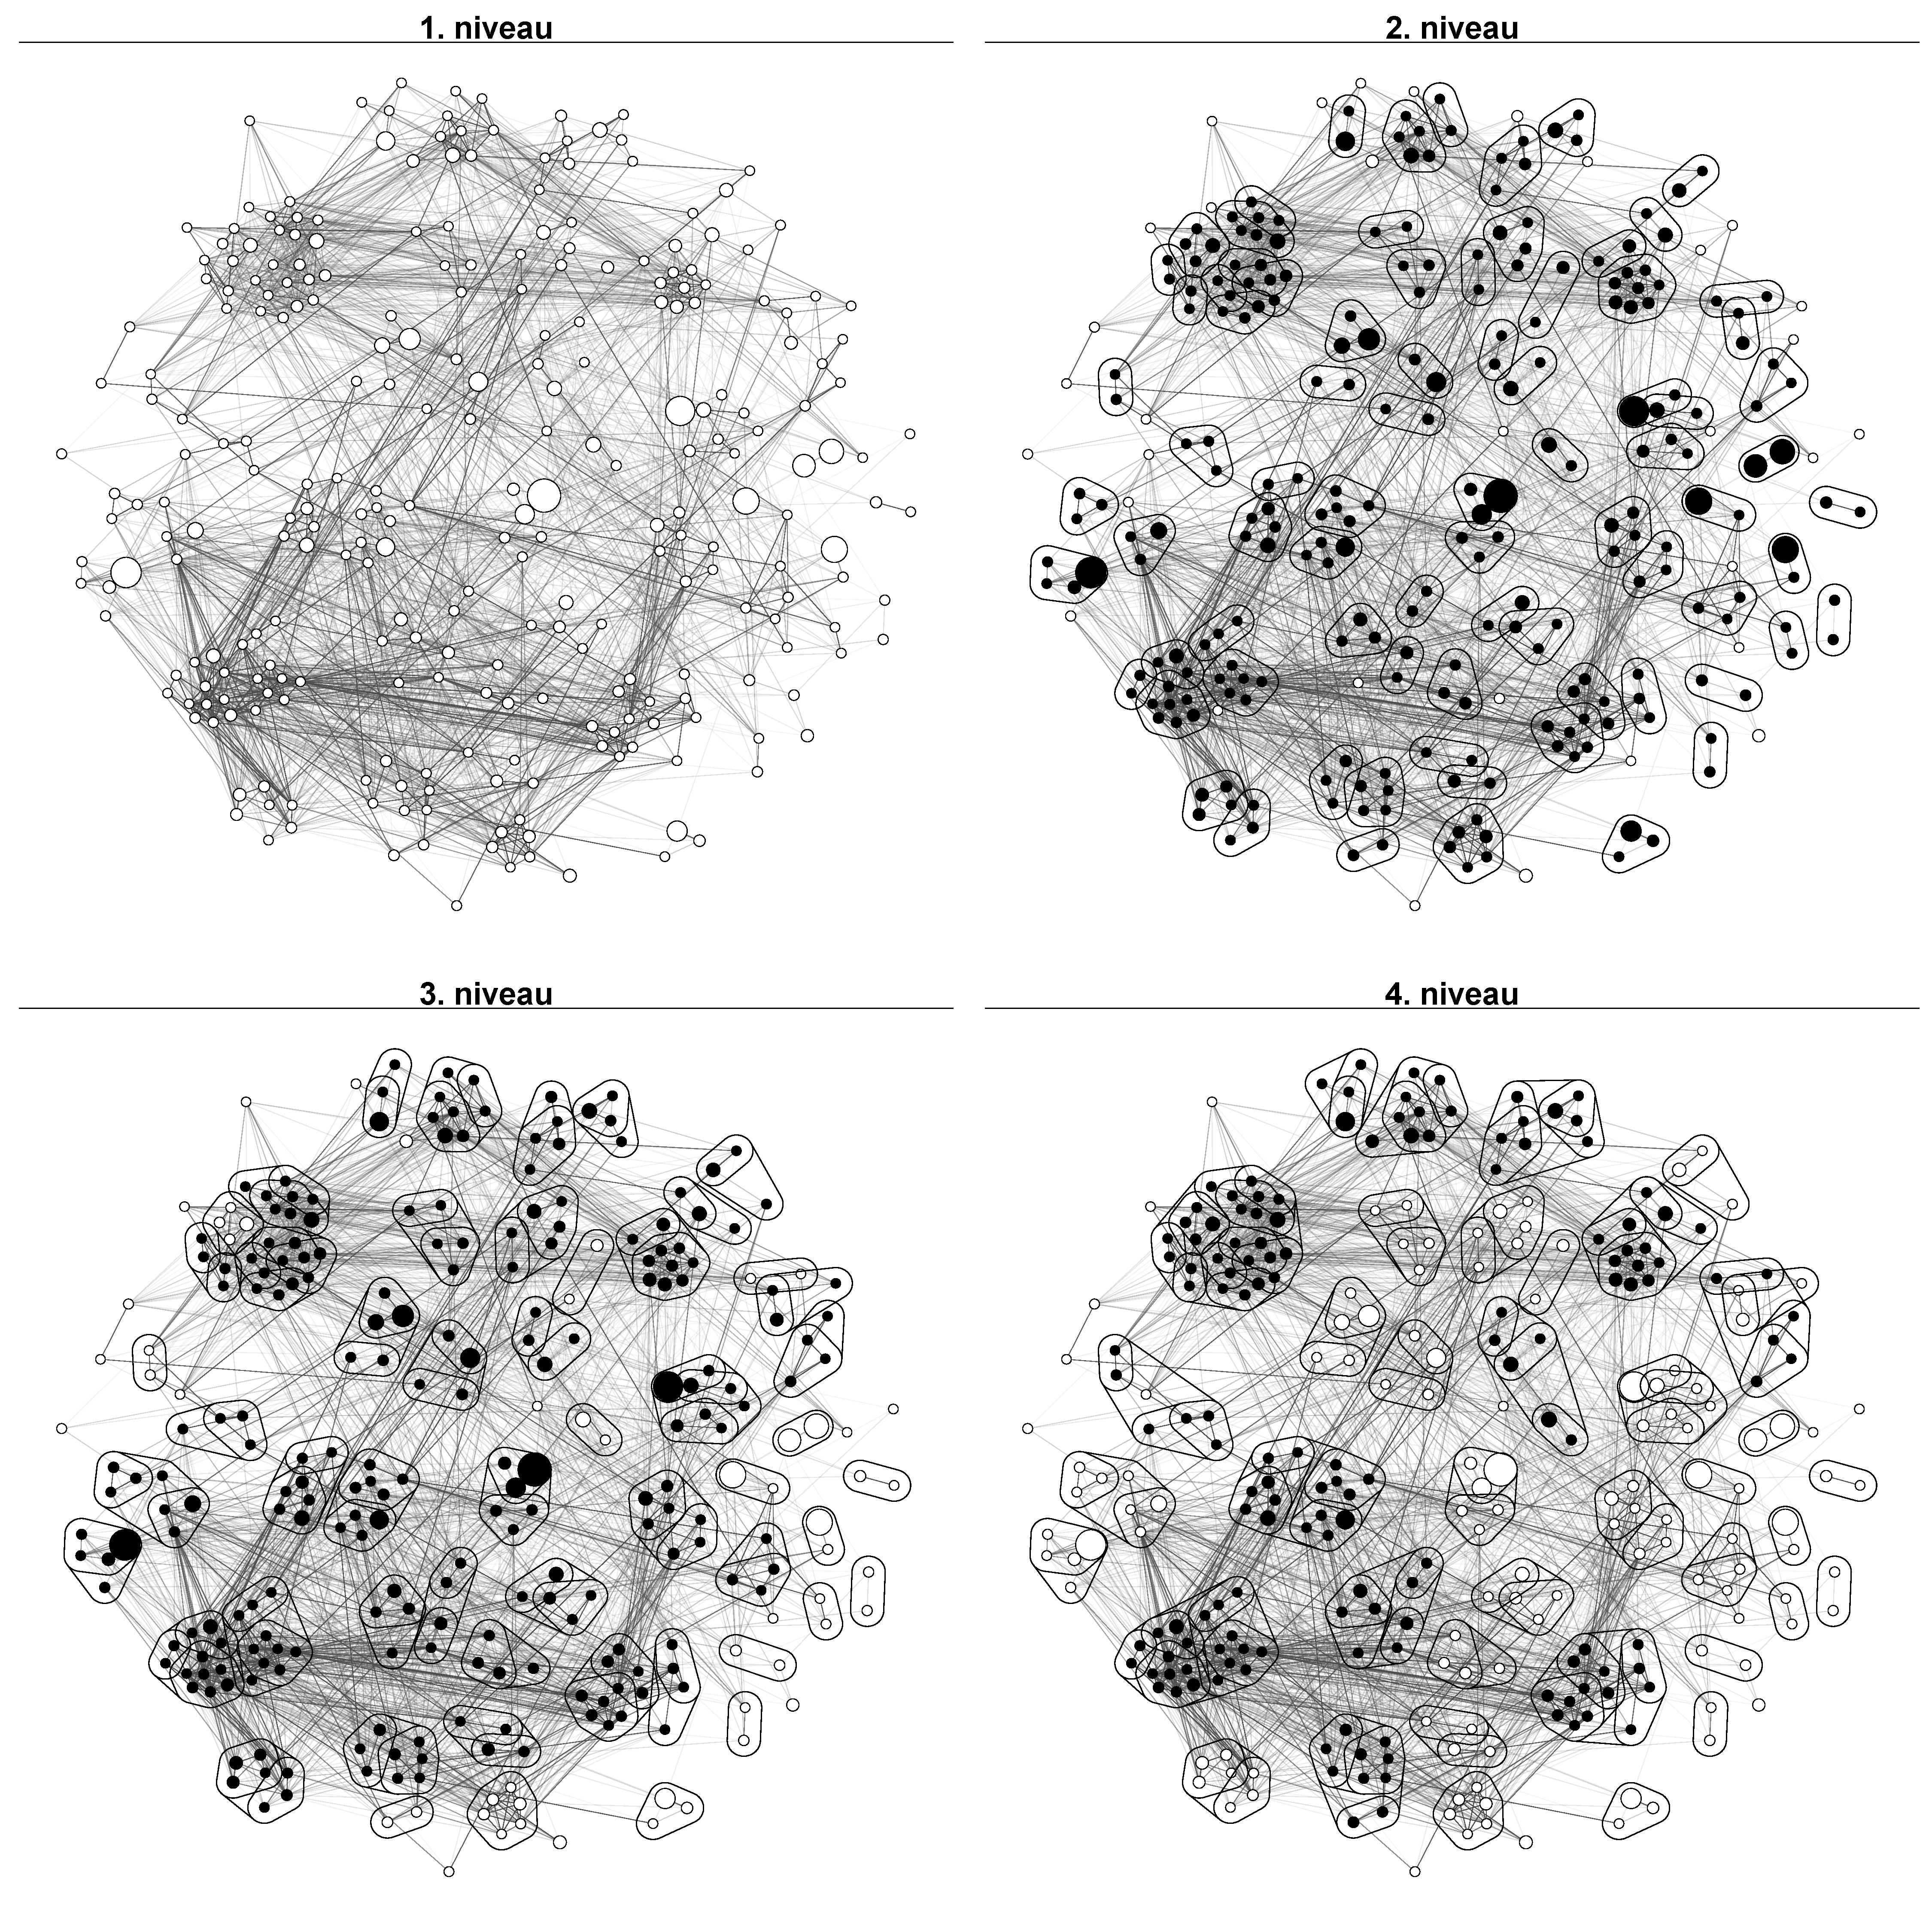
\includegraphics[width=1.0\textwidth]{fig/netvaerkskort/kort_seg_proces.pdf}
	\centerline{ \tiny{Kilde: Nielsen-Gravholt og Begtrup-Bright}}
\end{center}
\end{figure}
\restoregeometry
%
%

%%%%%%%%%%%%%%%%%%%%%%%%%%%%%%%%%%%%%%%%%%%%%%
\section{Den interne mobilitet i segmenterne \label{analyse_deskriptivt_within_mob_seg}}
%%%%%%%%%%%%%%%%%%%%%%%%%%%%%%%%%%%%%%%%%%%%%%


Det første netværkskort, jeg vil præsentere, er kortet der viser den interne mobilitet for hvert segment,  i figur \ref{fig_analyse_deskriptivt_kort_intern_mob_seg}, \pref{fig_analyse_deskriptivt_kort_intern_mob_seg}). % Den interne og eksterne mobilitet er drøftet teoretisk i afsnit ?? og den metodiske implementering er drøftet i afsnit ?? \#todo.
Da dette er det første kort, vil jeg først præsentere en vejledning i at læse de informationer, kortet indeholder. 

Noget man måske ligger mærke til ved første øjekast, er forbindelsernes farve og størrelsen af noderne. Som beskrevet i afsnit \ref{metode_relativrisiko}, er forbindelsernes styrke målt ved den relative risiko. Et forholdsmål, der udtrykker mobiliteten fra en kategori til en anden, givet den relative størrelse af antallet af beskæftigede i kategorien. Det er styrken af denne relative risiko, der afgør farven på forbindelserne: Helt lysegrå angiver en relativ risiko på 3, og helt orange angiver en relativ risiko på 15 eller derover. For at minde læseren om fortolkningen af relativ risiko (RR):  det vil sige, at der er ved en lysegrå forbindelse er 3 gange så stor sandsynlighed for mobilitet fra den forladte beskæftigelse til den nye beskæftigelse, i forhold til hvis der var tale om et helt frit arbejdsmarked. I bestemmelsen af klyngerne, er alle forbindelser med en RR på over 1 medtaget som en forbindelse. På det visuelle kort ville alle disse forbindelser ikke være til meget hjælp, da de mange pile og grå streger gør det umuligt at aflæse den underliggende systematik i hvilke forbindelser, der værd at lægge mærke til. Derfor visualiseres kun forbindelser med en RR på over 3. 

Argumentet for at vælge at sætte grænsen opadtil på 15, det vil sige reducere alle forbindelser med en RR på \emph{over} 15 \emph{til} 15 er anderledes. Her skyldes det at RR-værdierne mellem beskæftigelserne har et bredt udfaldsrum. (hvor bredt? kan du finde ud af det? \#todo) hvilket ikke er uinteressant, men repræsenteret som farvetoning på kortet, er en loyal repræsentation af denne skala ikke til meget hjælp. Visuelt er det svært at fortolke kompleksiteten, så i stedet har jeg valgt at alle RR-værdier over 15 - og der er mange - bliver sat \emph{til} 15. Derfor skal den rene orange farve tolkes ikke \emph{som} 15, men som “meget stærk” mobilitet fra en RR-værdi på 15 og op.

Størrelsen på noden repræsenterer ganske simpelt hvor mange personer, der i gennemsnit er i beskæftiget indenfor jobkategorien i årrækken 1996-2009%
%
\footnote{Når jeg fra nu af taler om hvor mange der er beskæftigede, vil det være underforstået at der er tale om det gennemsnitlige antal \emph{indenfor årrækken 1996-2009}, med mindre det eksplicit fremhæves at der er tale om noget andet.}%
%
. Ligesom med forbindelsernes styrke, er der ikke tale om et korrekt repræsenteret størrelsesforhold mellem de forskellige jobkategorier. Den største kategori, \texttt{5220: Ekspedient-, kasse- og demonstrationsarbejde} indeholder 114.869 personer i gennemsnit, svarende til 4,9 \% af det totale antal beskæftigede. Mens den mindste, \texttt{7346: Serigrafisk arbejde} indeholder 504 personer, svarende til 0,02 \% af det totalen. Det er for komplekst til visuel afkodning i et allerede informationstungt netværkskort, da de mindste noder ville blive meget små og de store noder voldsomt store. Derfor har jeg valgt et størrelsesforhold mellem noderne, der ikke er 1:1 med deres reelle forskelle i størrelse, men som alligevel giver en fornuftig fornemmelse for de reelle størrelsesforhold.  

Man skal dermed se både farve af forbindelserne og nodernes størrelse som en grov målestok af den variabel, den repræsenterer. Med vægten lagt på nem visuel afkodning, fremfor korrekt gengivelse af dataens reelle kompleksitet. Forbindelsernes styrke og beskæftigelseskategoriernes størrelse vil blive gennemgået nærmere senere, her præsenteres de kun med det formål at kunne aflæse kortene.  

Til sidst skal læseren mindes om, at der er tale om et retningsbestemt netværk, hvor pilene på kortet angiver retningen af mobiliteten mellem noderne. 

Det var de generelle retningslinjer for kortene. Dette gælder alle de præsenterede kort. Næste side indeholder(??) det første kort, der er farvelagt efter den interne mobilitet på segmentniveau.


\newgeometry{left=-0.01cm,bottom=0.1cm}
\begin{figure}[H]
\begin{center}
	\caption{Intern mobilitet for segmenterne.}
	\label{fig_analyse_deskriptivt_kort_intern_mob_seg}
	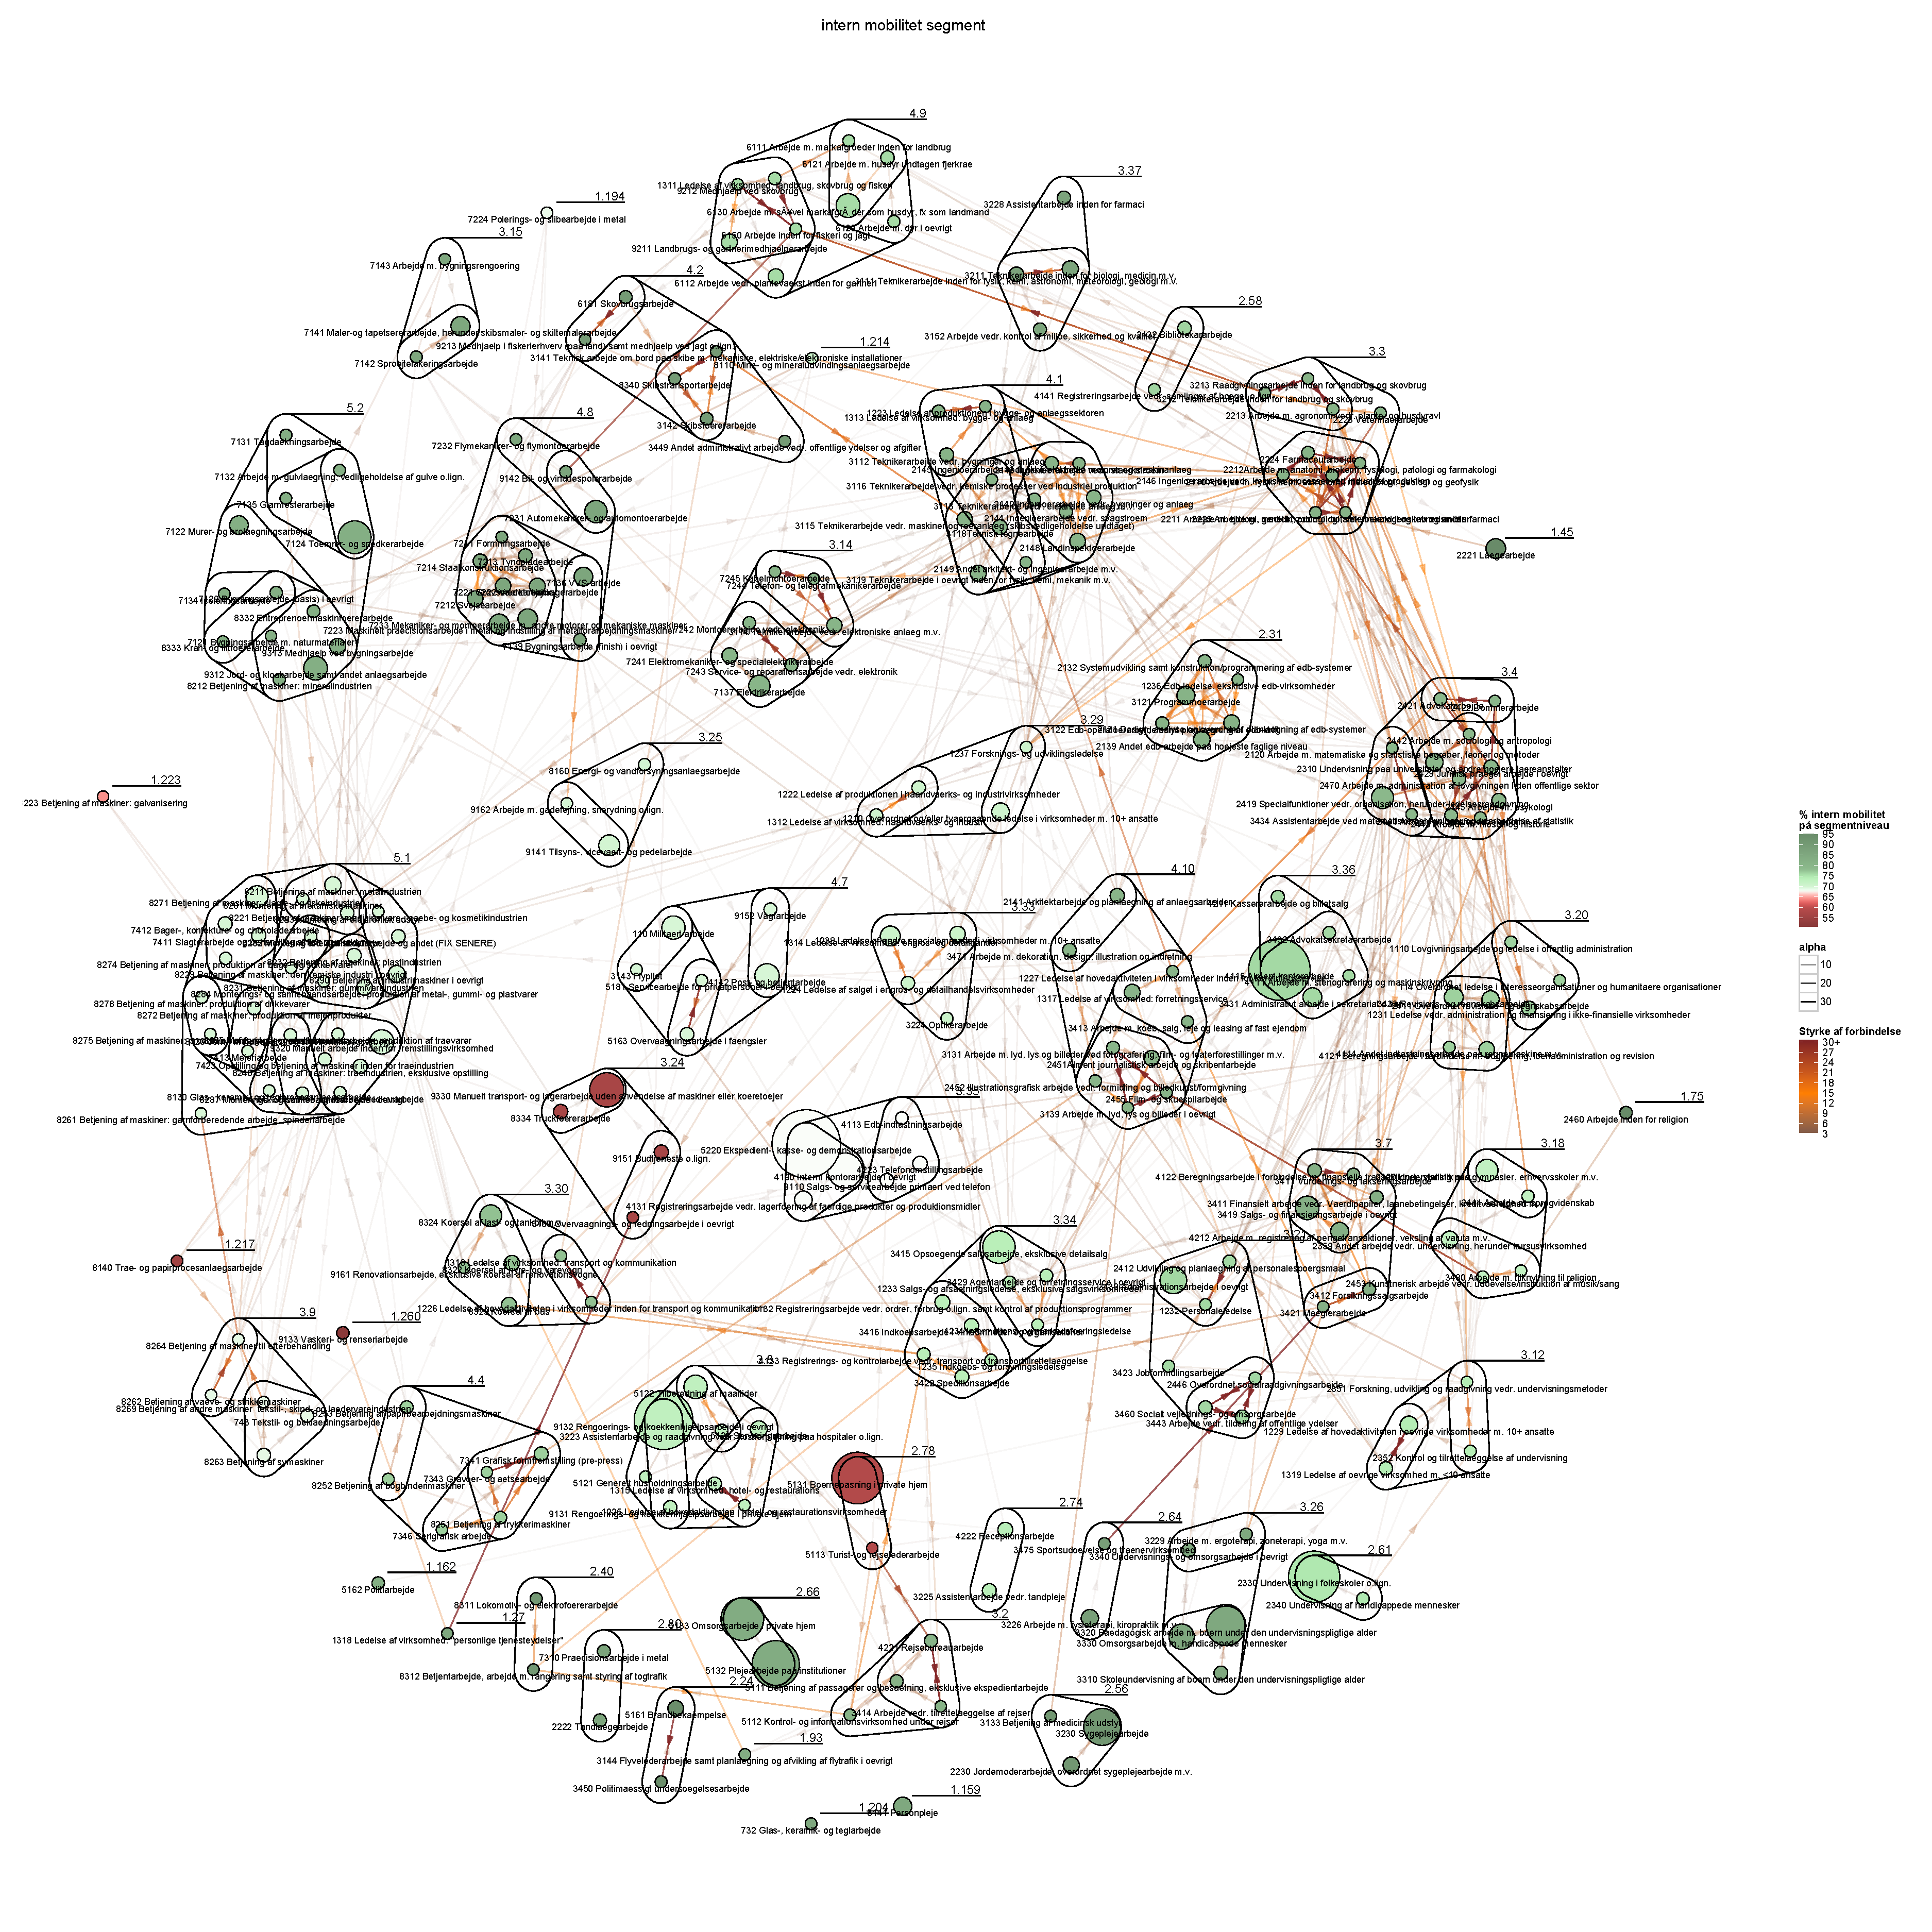
\includegraphics[width=1.0\textwidth]{fig/netvaerkskort/kort_intern_mob_seg.pdf}
	\centerline{ \tiny{Kilde: Nielsen-Gravholt og Begtrup-Bright}}
\end{center}
\end{figure}
\restoregeometry

Det ses på kortet, at nodernes farve går fra mørkerød, til hvid, til mørkegrøn. Mørkerød betyder at klyngen har en intern mobilitet på mellem 50 og 60 \%, mens den derfra og op til 69 \% antager en stadigt svagere lys rød, indtil den er ren hvid ved 70 \%. Derfra og op til 78 \% bliver den stadig mere grøn, for ved 80 \% at være helt mørkegrøn. Da der er tale om en gradient, er skiftet i farve ikke diskret, men kontinuert. 

Skiftet i farve er motiveret af min egen vurdering. Der findes ingen tidligere brug af Moneca algoritmen, hvori dette indgående bliver analyseret. Jeg har derfor besluttet mig for, at en mobilitet mellem erhvervene i en klynge på 70 \% og derover, er en fornuftig tærskel at benytte til at  vurdere kvaliteten af et segment, på dette parameter. Det ses at langt de fleste klynger overholder denne beslutningsregel. Klynge \emak{s5.1} har en intern mobilitet på 69,4 \%. Jeg vil betragte det som acceptabelt, da det ligger så tæt på min tærskelværdi. Der er ikke er tale om en statistisk test med et vist signifikansniveau, men min egen tentative vurdering. Og selv med de vedtagne signifikansniveauer i statistiske test, eksempelvis p-værdier i en T-test eller en F-test,  der advarer litteraturen om ikke at tolke disse tærskelværdier som skrevet i sten, men som nyttige konventioner (find henvisning, Gujarati og Malchow-Møller \#todo). 

Der kan være to årsager til lav intern mobilitet. Den ene er at beskæftigelserne i disse klynger simpelthen er jobs, der af den ene eller anden årsag er af en type, hvor folk sjældent opholder sig længe i dem. Det kunne være ufaglærte jobs, der typisk henvender sig til unge og studerende. Eller ufaglært, sæsonbetinget arbejde, eller jobs der simpelthen er så hårde, eller ansættelserne så usikre, at man ikke bliver i dem længe af gangen. Hvis arbejdet har denne karakter, må man forvente, at de sociale lukningsmekanismer næppe er særlig højtudviklede, hvoraf den mest legitime i moderne samfund må være adgangsgivende uddannelse. Vi vil derfor forvente at finde enten ufaglærte eller fag med lave uddannelsesmæssige krav. 

Hvis vi kigger på klynge \emak{s2.78}, kan vi se at den består børnepasning i private hjem, samt turist- og rejseledere, der har en intern mobilitet på henholdsvis  59 \% og 47 \%, altså ganske lavt sammenlignet med den gennemsnitlige interne mobilitet indenfor erhvervene selv, der er på 68 \%.  Begge jobs er indenfor hovedgruppe 5 i Disco-nomenklaturet, salgs-, service- og omsorgsarbejde. Det er arbejde, der ifølge Danmarks Statistik er klassificeret som ISCEDs færdighedsniveau 2, hvilket betyder at det kræver uddannelse “på grundniveau” \parencite[tabel 1]{DSTDISCO88}. Det er en klar indikator på at de formelle sociale lukningsmekanismer i erhvervene er begrænsede. 


Der er imidlertidig også andre klynger på kortet, hvor uddannelseskravene er lave, men hvor den interne mobilitet er høj. Et nærliggende eksempel er klynge \emak{s2.66}, Der ligeledes befinder sig i hovedgruppe 5, men hvor den interne mobilitet både i klyngen og blandt jobbene selv er meget høj. Børnepasning i private hjem ligger ganske tæt på arbejdsfunktionerne i klynge \emak{s2.66}, faktisk så tæt at de også på et 3-cifret Disco niveau er kategoriseret ens. Men børnepasning i private hjem har tilsyneladende en noget anden social profil. Den interne mobilitet er meget lavere, og den ligger sammen med turist- og rejseleder. 

Det ses også at der ikke er nævneværdig mobilitet mellem de to klynger, trods denne enshed. Det får mig til at konkludere, at der trods en vis funktionel enshed mellem børnepasning på en ene side og omsorgsarbejde for ældre mennesker i deres hjem og på institutioner på den anden, er tale om vidt forskellige sociale processser. Den funktionelle enshed er ikke bestemmende for den sociale ditto. Det viser sig også ved at gennemsnitlige alder indenfor klynge \emak{s2.78} er omtrent 37 år.%
%
\footnote{Det også gælder de to jobs i klyngen hver især}%
%
. Klynge \emak{s2.66} har en gennemsnitsalder på 42 $\nicefrac{3}{4}$ år, hvilket er er nærmest identisk med populationsgennemsnitet på 42,3 år. (check hvilken kvartil det befinder sig i på forskermaskinen \#todo). 


















%%%%%%%%%%%%%%%%%%%% noter %%%%%%%%%%%%%%%%%%%%%%%%%%%%%%%%%%%%%%%%%%%


%  Måske skal der laves mere stringent begrebsafklaring om forskel på delmarkeder, segmenter og klynger. 


